
\chapter{Governing equations and finite element formulations}\label{cha:governing_equations}
The following section provides a short summary of the most important equations of solid mechanics in the finite element context. It thus serves as a short preparation for Chapter \ref{cha:feti_formulation}, which will will enhanced the basic formulation by a domain decomposition approach. A comprehensive declaration of all terms and expressions used in this thesis can also be found in the nomenclature. Moreover, since domain decomposition typically involves some kind of constraint enforcement, the most important methods in a finite element context are highlighted.
\section{Solid mechanics}\label{sec:solid_mechanics}

The classical displacement based problem in linear continuum mechanics can be described by a set of three governing equations. The balance equation(BE) describes the relationship between the stress resultant and the external forces, the constitutive equation(CE) provides information about the material behaviour and finally, the kinematic equation (KE) links displacement and strains.
The basic equations can be very descriptively linked in the Tonti diagram\cite{Tonti2013}, as provided in Figure~\ref{fig:tonti}.\\
\begin{figure}[h]
  \centering
  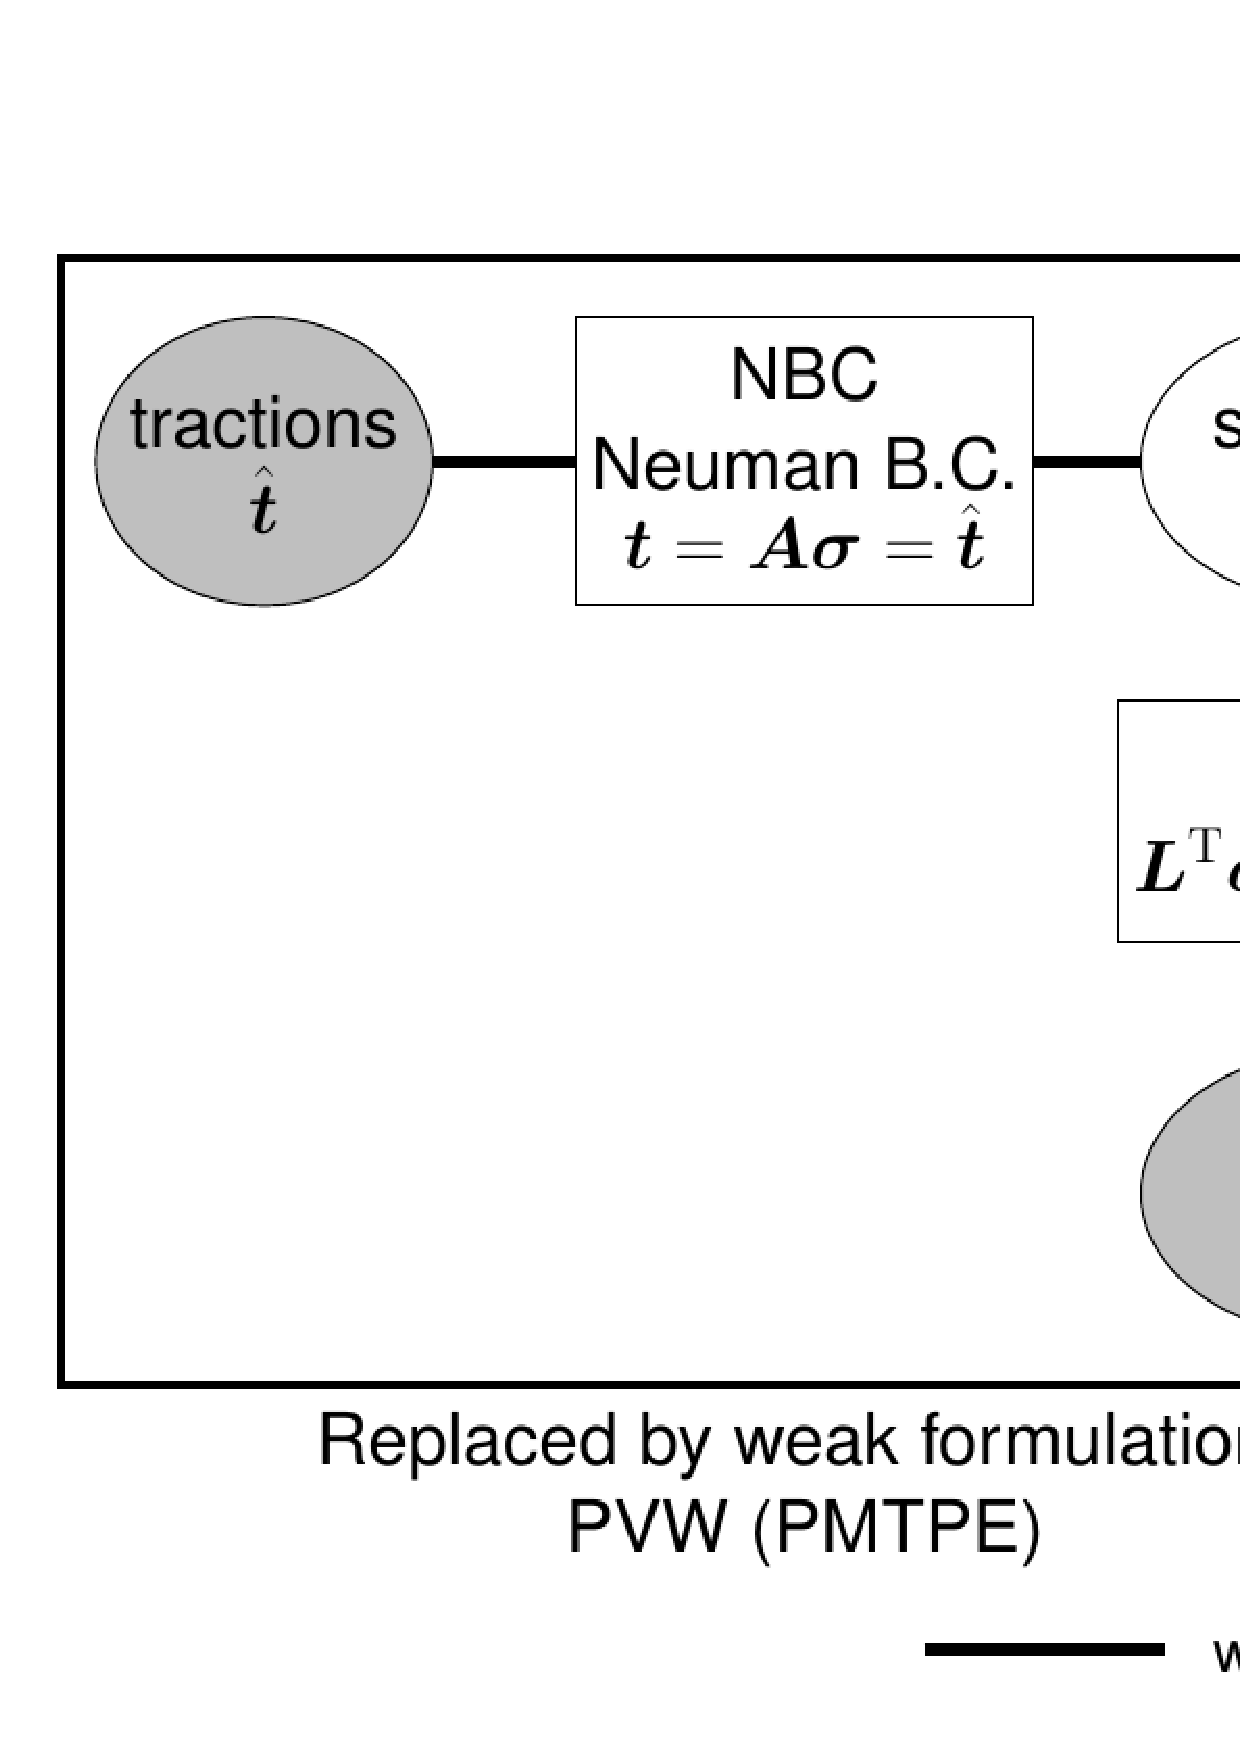
\includegraphics[width=0.8\textwidth]{./fig/pdf/tonti.pdf}
  \caption[Tonti diagram linear]{Tonti diagramm for a linear, small displacement elasticity problem. It classifies variables and equations of the solid mechanics PDEs and helps to derive an appropriate finite element formulation. A classic, displacement based formulation is depicted here.}\label{fig:tonti}
\end{figure} \\
\\
In index-notation, the system of equations to be solved reads
\begin{align}
    & \frac{\partial}{\partial x_i} \sigma_{ij} + \bar{X_j}=0 & in~\Omega_0           \\
    & t_j=n_i \sigma_{ij} = \bar{t}_j                         & on~Neumann~ boundary  \\
  &\sigma_{ij}=\sigma_{ji}\\
  &\sigma_{ij}=C_{ijkl} \epsilon_{kl}\\
  &\epsilon_{ij}=\frac{1}{2} (\frac{\partial u_j}{\partial x_i}+\frac{\partial u_i}{\partial x_j}) \\
    & u_j = \bar{u}_j                                         & on~Dirichlet~boundary 
\end{align}
\\
A system of equations is derived, that can, except for special, very simple cases, not be solved analytically.\\
The finite element method now entails two key ideas. Firstly, instead of a continuous domain, considerations are focused on a finite number of discrete elements("finite elements"). Each Element defines its own function space for the primary variables via the so called shape functions. It is obvious that the thereby introduced limitation of the solution function space will generally not contain the solution to the original problem.  Therefore, as a second step, selected governing equations are "weakened", i.e. they are multiplied by a weighting function and only enforced in an integral sense. For the formulation, presented in Figure~\ref{fig:tonti} the weak form can be formulated as

\begin{align}
  \int_{\Omega}  \underbrace{(\nabla \cdot \stress^{\disp} + \bodyforce)}_{\vec{R}_\mathrm {BE}} ) \cdot \underbrace{\vec{w}}_{\substack{\text{weighting}       \\\text{function}}}~d\Omega +
  \int_{\Gamma_\sigma}  \underbrace{(\nabla \cdot \stress^{\disp} + \bodyforce)}_{\vec{R}_\mathrm{FBC}} )\cdot \underbrace{\vec{w}}_{\substack{\text{weighting} \\\text{function}}}~d\Gamma
  =0~. \label{eq:weighted_residuals}                                                                                                                            
\end{align}


Gauss divergence divergence is subsequently applied for further derivations.
%
\paragraph{Principle of Virtual Work}
Generally, the weight function $\vec{w}$ is arbitrary, and can be chosen freely. If, however, one makes the particular choice of
\begin{align}
  w_\mathrm{i}=\pd u_\mathrm{i} 
\end{align}
work expressions are obtained for the individual terms and the Principle of Virtual Work~(PVW) is derived as (in matrix notation)
\begin{align}
  \int_\Omega \pd \strain^{\disp \mathrm T} \stress^{\disp}~d\Omega                   
  =                                                                                   
  \int_\Omega \pd \disp^{\mathrm T}~d\Omega                                           
  +                                                                                   
  \int_{\Gamma_\sigma} \pd \disp^{\mathrm T} \traction~d\Gamma~. \label{eq:solid_PVW} 
\end{align}


The PVW is valid for arbitrary materials, also for dissipative ones that have no potential.
The finite element formulation is finally derived expressing all terms of the PVW exclusively in the primary variables. To do so, the strong connections of the Tonti diagram are taken advantage of.

\section{Space discretization}\label{sec:space_discretiaztion}
The FEM in solid mechanics is based upon the idea of finding a numerical solution to Equation~\eqref{eq:general_problem_FE} at discrete points, commonly referred to as nodes. Connected nodes form elements, into which the problem domain is partitioned into:
The primary variable on element $e$ is then typically approximated by interpolation functions ~( shape functions ).\\
In this case, the displacement field has been used as the only primary variable, and a local interpolation approach, i.e., the shape functions only have local support, has been utilized.\\
Therefore:
\begin{align}
  \Omega_\mathrm 0   & \approx\cup_\mathrm {e=1}^{nele} \Omega_\mathrm 0^{(e)}~, \\
  \disp(\vec{X},t)   & \approx                                                   
  \disp_\mathrm h^{(e)}(\vec{X},t)=
  \sum_\mathrm {k=1}^{nnod^{(e)}} N_\mathrm k(\vec{X}){d}_\mathrm k(t)~. \label{eq:fe_interpolation} \\
  \vec{x}(\vec{X},t) & \approx                                                   
  \vec{x}_\mathrm h^{(e)}(\vec{X},t)=
  \sum_\mathrm {k=1}^{nnod^{(e)}} N_\mathrm k(\vec{X}){x}_\mathrm k(t)~. \label{eq:fe_interpolation}
\end{align}


\section{Methods of constraint enforcement}\label{sec:constraint_enforcement}
From a mathematical point of view, coupling problems are basically optimization problems with equality constraints. A problem of this kind can generally be formulated as:
\begin{align}\label{eq:optimization_problem}
  \underset{x}{\text{min}}~ & \vec{f(x)}~,   \\
  \text{subjected to }      & \vec{g(x)}=0~. 
\end{align}
Numerous methods have been proposed to solve this kind of problems. Among the most common ones are the Lagrange multiplier approach and the penalty method. This thesis focuses solemnly on the first on, nevertheless a quick introduction into the alternatives shall be provided, so that the pros and cons of each method can be discussed.
\subsubsection{Lagrange multiplier approach}\label{sec:lagrange_multiplier_approach}
The Lagrange multiplier method demands the existence of continuous partial derivatives for both: $\vec{f}$ and $\vec{g}$. It introduces a new variable $\lagvec$, called Lagrange multiplier, and considers the Lagrange function defined as
\begin{align}
  \Lambda(\vec{x},\vec{\lambda})=\vec{f(\vec{x})}+\lambda\cdot\vec{g(\vec{x})}~. 
\end{align}
\\
Solutions of the original problem are stationary points of the Lagrange function. However, not all stationary points yield a solution of the original problem. The method of Lagrange multipliers thus gives a necessary condition. Sufficient conditions can be obtained by surveying the Hessian matrix. Details can be found in any standard mathematical literature concerning optimization theory.
The main advantage of the Lagrange multiplier approach lies in its exact fulfilment of the constraints. Moreover, it is a single step method, meaning that no iterative procedure is necessary to fulfil the boundary conditions.\\
The Lagrange multiplier approach does, however, come with the disadvantage of introducing additional unknowns, as well as worsening the overall system of equations constitution.
\subsubsection{Penalty approach}
A penalty method replaces the constraint problem by a series of unconstrained problems, such that their solutions ideally converge to the solution of the original problem. Basically the series of unconstrained minimization problems can be written as:
\begin{align}
  \text{min}~\Phi(\vec{x}) & =f(\vec{x})+\sigma_\mathrm k \sum_\mathrm {i \in I} g(c_\mathrm i(\vec{x})),~\text{where} \\
  g(c_\mathrm i(\vec{x}))  & = \text{min}(0,ci(x))^2~.                                                                 
\end{align}
They main advantage of the penalty method lies in the fact, that it does not introduce any new unknowns, and thus maintains the positive definiteness of the system matrix. On the other hand, the constraints are not fulfilled exactly. Regarding the choice of $\sigma_\mathrm k$ one has to weight carefully between a more accurate constraint fulfilment and the overall systems constitution since a greater $\sigma_k$ value might enforce the constraints stronger, but can also lead to numerical instabilities.
\subsubsection{Augmented Lagrange}
The Augmented Lagrange method has similarities to the Penalty method. It replaces the constraint optimization problem by a series of unconstrained problems and adds a penalty term to the objective. Moreover, the Augmented Lagrange Method adds yet another term, that mimics a Lagrange multiplier.\\
Starting from the problem defined in Equation~\eqref{eq:optimization_problem}, the approach uses the following unconstrained objective:
\begin{align}
  \mathrm{min}~\boldsymbol{\phi}_\mathrm{k}(\vec{x})=f(\vec{x})+\frac{\mu_\mathrm{k}}{2} \sum_{i\in I} g(c_i)(\vec{x})^2 - \sum_{i\in I} \lambda_i g(c_i)(\vec{x})~. 
\end{align}
After each iteration, not only $\mu_k$, but also the variable $\lambda$ is updated according to the rule
\begin{align}
  \lambda_i \leftarrow \lambda_i-\mu_k c_i(\vec{x}_k)~, 
\end{align}
where $\vec{x}_k$ denotes the solution to the unconstrained problem at the k-th step.\\
The variable $\lambda$ can be regarded as an estimate of the Lagrange multiplier, as introduced in Section~\ref{sec:lag_approach}.\\
Contrary to the Penalty approach, $\mu \rightarrow \infty$ is not required in order to solve the original, unconstrained problem, thanks to the presence of the Lagrange multiplier term. The method is therefore especially favourable due to both, an exact fulfilment of the boundary conditions and no introduction of new Unknowns. It also avoids the ill conditioning of the standard quadratic penalty method.
\subsubsection{Nitsche method}\label{sec:nitsche_method}
The Nitsche Method is closely related to the development of discontinuous Galerkin methods. It has originally been developed as a simple approach to handle Dirichlet boundary conditions, but its real strength lies in the generality with which interface problems can be handled: arbitrary degree of polynomial approximations, arbitrary( shape regular meshes ), even different physical models on either side are possible~\cite{Hansbo2005}.\\
A full introduction is beyond the  scope of this thesis, thorough investigations are provided in~\cite{Nitsche1971} and~\cite{Hansbo2005}.\\